\documentclass[a4j,12pt,]{jarticle}
 \usepackage[dvipdfmx]{graphicx}
 \usepackage{float}
 \usepackage{siunitx} %%SI単位系用
 \usepackage{amssymb, amsmath}
 \usepackage{ascmac,here,txfonts,txfonts}
\usepackage{listings,jlisting}
\usepackage[dvipdfmx]{color}
\lstset{%
  language={Python},
  basicstyle={\small},%
  identifierstyle={\small},%
  commentstyle={\small\itshape\color[rgb]{0,0.5,0}},%
  keywordstyle={\small\bfseries\color[rgb]{0,0,1}},%
  ndkeywordstyle={\small},%
  stringstyle={\small\ttfamily\color[rgb]{1,0,1}},
  frame={tb},
  breaklines=true,
  columns=[l]{fullflexible},%
  numbers=left,%
  xrightmargin=0zw,%
  xleftmargin=3zw,%
  numberstyle={\scriptsize},%
  stepnumber=1,
  numbersep=1zw,%
  lineskip=-0.5ex%
}
\begin{document}

{\noindent\small 第4回報告書 \hfill\today}
\begin{center}
  {\Large 任意の緯度経度と日時から日射量を計算するプログラムの開発}
\end{center}
\begin{flushright}
  祖父江匠真 \\
\end{flushright}

\section{はじめに}
CSVデータなどで保存された太陽光発電の環境データはオフライン環境でファイル書き込みを行っているため, PCの内部時計がずれており日時情報が誤っている場合がある.
そこで, 任意の緯度経度と日射量から日時を求めることの第一段階として, 任意の緯度経度と日時から日射量を計算するプログラムを開発した.

\section{日射量の式の導出}
任意の緯度経度, 日時における日射量$Q$は, 任意の緯度$\phi$, 経度$\lambda$の地点における任意の日時, 太陽高度$\alpha$から求めることができる.

まず, 次式により元旦からの通し日数$dn$に基いて定めた$\theta$を用いて, 当該日の太陽赤緯$\delta$, 地心太陽距離$\frac{r}{r^{*}}$, 均時差$E_q$をそれぞれ以下の式により求める.
\begin{eqnarray}
  \theta =  \frac{2\pi (dn-1)}{365}
\end{eqnarray}

\begin{eqnarray}
\begin{split}
  \delta =  0.006918-0.399912\cos \theta+0.070257\sin \theta-0.006758\cos 2\theta\\
  +0.000907\sin 2\theta-0.002697\cos 3\theta+0.001480\sin 3\theta
\end{split}
\end{eqnarray}

\begin{eqnarray}
  \frac{r}{r^{*}} =  \frac{1}{\sqrt{1.000110+0.034221\cos \theta+0.001280\sin \theta+0.000719\cos 2\theta+0.000077\sin 2\theta}}
\end{eqnarray}

\begin{eqnarray}
  E_q =  0.000075+0.001868\cos \theta-0.032077\sin \theta-0.014615\cos 2\theta-0.040849\sin 2\theta
\end{eqnarray}

日本標準時間から, 太陽の時角$h$を求める.

\begin{eqnarray}
  h = \frac{(日本標準時間-12)\pi}{12}+標準子午線からの経度差+E_q
\end{eqnarray}

$\delta$, $\phi$, $h$の値が既知となったので$\alpha$は

\begin{eqnarray}
  \alpha = \arcsin (\sin \phi\sin \delta+\cos \phi\cos \delta\cos h)
\end{eqnarray}

として求めることができる.

最後に, $Q$を

\begin{eqnarray}
  Q = 1367(\frac{r^{*}}{r})^{2}\sin \alpha
\end{eqnarray}

により求めることができる.
また, 1367\si{\watt}/\si{\metre\squared}は太陽定数である.

\section{日射量を計算するプログラムの開発}
式(1)から式(7)をもとに開発した日射量を求めるプログラムをソースコード\ref{sc1}に示す.
なお, ソースコード\ref{sc1}では式(7)の計算について, 式変形によって得られた以下の式(8), (9)を用いて計算している.

\begin{eqnarray}
  (\frac{r^{*}}{r})^{2} = 1.000110+0.034221\cos \theta+0.001280\sin \theta+0.000719\cos 2\theta+0.000077\sin 2\theta
\end{eqnarray}

\begin{eqnarray}
  \sin \alpha = \sin \{\arcsin (\sin \phi\sin \delta+\cos \phi\cos \delta\cos h)\} = \sin \phi\sin \delta+\cos \phi\cos \delta\cos h
\end{eqnarray}

\begin{lstlisting}[caption=任意の緯度経度と日時から日射量を計算するプログラム, label=sc1]
import numpy as np
import datetime

dt = datetime.datetime(2022, 5, 17, 17, 53)
dt_new_year = datetime.datetime(dt.year, 1, 1)
dt_delta = dt - dt_new_year  # 元旦からの通し日数

dn = dt_delta.days + 1
theta = 2 * np.pi * (dn - 1) / 365

# 太陽赤緯(単位はラジアン)
delta = (
    0.006918
    - (0.399912 * np.cos(theta))
    + (0.070257 * np.sin(theta))
    - (0.006758 * np.cos(2 * theta))
    + (0.000907 * np.sin(2 * theta))
    - (0.002697 * np.cos(3 * theta))
    + (0.001480 * np.sin(3 * theta))
)

# 地心太陽距離のルートの中身
geocentri_distance_like = (
    1.000110
    + 0.034221 * np.cos(theta)
    + 0.001280 * np.sin(theta)
    + 0.000719 * np.cos(2 * theta)
    + 0.000077 * np.sin(2 * theta)
)

eq = (  # 均時差
    0.000075
    + 0.001868 * np.cos(theta)
    - 0.032077 * np.sin(theta)
    - 0.014615 * np.cos(2 * theta)
    - 0.040849 * np.sin(2 * theta)
)

lng_deg = 132.75093  # 任意の経度(longitude)
lng_rad = lng_deg * np.pi / 180

lat_deg = 33.82794  # 任意の緯度(latitude)
phi = lat_deg * np.pi / 180

lng_diff = (lng_deg - 135) / 180 * np.pi  # 経度差


def calc_h(dt, lng_diff, eq):
    return (dt.hour + dt.minute / 60 - 12) / 12 * np.pi + lng_diff + eq


# 太陽高度のarcsinの引数になる値
def calc_sun_altitude_like(h, delta, phi):
    return np.sin(phi) * np.sin(delta) + np.cos(phi) * np.cos(delta) * np.cos(h)


h = calc_h(dt, lng_diff, eq)  # 時角

sin_alpha = calc_sun_altitude_like(h, delta, phi)
print(f"日射量:{1367*geocentri_distance_like*sin_alpha}")
\end{lstlisting}

ソースコード\ref{sc1}では, 2022年5月17日17時53分0秒における, 経度132.75093, 緯度33.82794の地点での日射量を計算している.
ソースコード\ref{sc1}を実行すると, 図\ref{p1}が出力される.
図\ref{p1}から, 今回与えた日時, 緯度経度における日射量は, 約299.15\si{\watt}/\si{\metre\squared}となった.

\begin{figure}[H]
  \begin{center}
    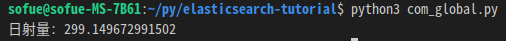
\includegraphics[width=160mm]{output.png}
    \caption{ソースコード\ref{sc1}の実行結果}
    \label{p1}
  \end{center}
\end{figure}

\section{おわりに}
今回は, 任意の緯度経度と日時から日射量を計算するプログラムを開発した.
次回は実際に測定したリサイクル館の日射量計測データと, 開発したプログラムによって計算した日射量を比較することで計算精度を検証する.

\begin{thebibliography}{5}
  \bibitem{1}中川清隆,"太陽方位、高度、大気外日射量の計算", http://www.es.ris.ac.jp/~nakagawa/met\_cal/solar.html,参照 May 23, 2022.
\end{thebibliography}

\end{document}